\chapter{Inside the VoiceP}\label{insidevp}
In this chapter, I will show that inner aspects, i.e., the aspects located below VoiceP, are systematically expressed via a manipulation of the verb sign (what I call `lower layering'\is{lower layering}). To show this, I will first repeat the main hypothesis guiding the first part of this chapter in Section \ref{inneraspects}. Then I will discuss what is called `habitual aspect' and `durative aspect' in the sign language literature, two categories which finds expression by lower layering. I will show that what is called habitual in the Cinquean system and what is called habitual in the sign language literature are in fact two different categories with two different scope positions. A similar point is made for durative aspect. Then, I will discuss the remaining Cinquean categories, namely inceptive aspect II (Section \ref{inceptivetwo}), continuative aspect II (Section \ref{continuativetwo}), celerative aspect II (Section \ref{celerativetwo}), completive aspect II (Section \ref{completivetwo}), repetitive aspect II (Section \ref{repetitivetwo}), and frequentative aspect II (Section \ref{frequentatitivetwo}). As there are not many categories left, this chapter is comparatively short.

%The two last parts of the chapter are devoted to the behavior and syntactic position of the direct object in DGS. In Section \ref{definiteness}, I will show that DGS exhibits object shift. While objects staying inside the VP receive an indefinite and unspecific interpretation, more definite and more specific direct objects have to move into a higher IP-internal position. In Section \ref{dom}, I will discuss the `person agreement marker' \textsc{pam}, a sign which is traditionally analyzed as an auxiliary verb and discuss evidence that it is in fact a differential object marker.

\largerpage
\section{The inner aspects}\label{inneraspects}\is{inner aspect}\is{aspect}

In the previous chapter I claimed that aspectual categories that are expressed via modulations of the movement or path of a verb sign are an expression of inner, and not outer, aspects. In other words, I claimed that aspects expressed by the addition of a bound morpheme belong to the class of aspects below Voice, labeled II by Cinque. This hypothesis is shown in (\ref{vpinternalmodhyp}), repeated here for convenience in (\ref{vpinternalmodhypa}).

\begin{exe}
\ex \textit{The VoiceP-internal modulation hypothesis:}\\
Aspectual categories below the VoiceP (the so-called `inner aspects') do not find their expression by adding manual signs, but by modulating the movement path of the verb sign. \label{vpinternalmodhypa}\is{VoiceP-internal modulation hypothesis}\is{inner aspect}
\end{exe}


\noindent In the next sections I will very briefly describe the empirical motivation of this claim for the so-called `habitual aspect', a category which can find expression through a manipulation of the movement path of the verb sign although it should be located inside the IP (as discussed in Section \ref{habitualaspect}) and what is often called `durative' (and sometimes also `continuative aspect'). The reasoning is rather simple: if an aspectual category is located inside the VoiceP it should not be possible for it to take scope over a higher-scoping category. After this, I will discuss the other lower VoiceP-internal aspects in Cinque's system. One problem with the present chapter is that there are many terminological distinctions in the literature and that often one label is used by different authors to refer to different categories and that sometimes different labels are used for the same category. Hence, there is a great deal of terminological confusion.

A last note concerns facial non-manuals used with inner aspects. There are some notes in the literature on such uses. \citet{hoitingslobin2001typological}, for example, note that continuative aspect II and habitual aspect are marked by the insertion of the manual sigh \textsc{through} (which itself shows manipulations of the movement path similar to the ones described in this chapter, namely reduplicated movements) in \is{Sign Language of the Netherlands}Sign Language of the Netherlands. However, the continuative is also accompanied by ``pursed lips and a slight blowing gesture'' while the habitual is accompanied by ``lax lips with protruding tongue'' \citep[127]{hoitingslobin2001typological}.

However, this analysis of continuative and habitual aspect in Sign Language of the Netherlands was challenged by \citet{oomen2016aspectual}, who did not find uses of the sign \textsc{through}, but only observed that the movement paths of the respective verb signs were manipulated as expected by the hypothesis put to test in this chapter. Additionally, she found ``synchronous back-and-forth movement of the head or body'' \citep[43]{oomen2016aspectual} which are probably performance phenomena due to the manipulation of the movement path of the verb sign. Additionally, \citet[17]{boven2018throughaspect} also disagrees with \citet{hoitingslobin2001typological} and concludes that ``none of the non-manual markers identified in previous studies are  used  consistently''.% This can be taken as evidence that the higher non-manuals are used to express structurally higher meanings.


Nevertheless, I assume that similar observations might be made for other sign languages (i.e., the observation of facial non-manuals with lower aspectual categories). There are two possible solutions to this. First, it might be that these lower-face non-manuals add a structurally high signer evaluation. In the case of the pursed lips, it might, for example, be that they are a reflection of the scalarity projection (see Section \ref{scalarity}).\is{scalarity} Similar to the evaluation found with the sign \textsc{just} (see Section \ref{justjust}). This analysis is backed up by \citeauthor{boven2018throughaspect}'s observation that the non-manuals described by \citet{hoitingslobin2001typological} are often absent. The second possibility would be that the connection facial non-manuals and structurally higher syntactic projections is not bidirectional, but unidirectional. This would mean that structurally higher projections lead to facial non-manuals, but that the use of facial non-manuals does not in any case mean that they are reflections of structurally high projections. I will leave this open for future research.


\section{The so-called `habitual aspect'}\label{habitualtwo}\is{habitual aspect|(}
In Section \ref{habitualaspect} I briefly discussed the fact that it is possible that in DGS habitual aspect is expressed via \is{reduplication}reduplication of the verb sign (this reduplication can be analyzed as attaching a bound habitual morpheme to the verb). This was illustrated by the example in (\ref{queretaldgs}), repeated here in (\ref{queretaldgsa}), from \citet[225]{signgram2017}.

\begin{exe}
\ex \textsc{saturday index\textsubscript{1} shopping go+++} (fast \& small repetitions)
\glt `I usually go shopping on Saturday.'\label{queretaldgsa}
\end{exe}

\noindent As the example shows, habitual aspect can find its expression via a modulation of the movement path of the verb sign (similar facts hold for other sign languages as well, see \citealt{wilbur2009productive} for \is{American Sign Language}American Sign Language). This contradicts the hypothesis in (\ref{vpinternalmodhypa}) according to which such a movement-path manipulation should be an expression of inner aspects inside the VoiceP -- habitual aspect, however, should be located higher up in the structure (inside the IP) and should thus be expressed by adding a manual sign (in this case, the sign \textsc{always} or \textsc{usually}).

One solution would be to claim that habitual aspect behaves like other aspectual categories and is split into habitual aspect I and habitual aspect II. The manual strategy then would express the higher habitual I and the movement-modulation strategy the lower habitual II. If this is correct, habitual II should not be able to scope over higher categories located outside the VoiceP. To be more precise, if habitual II was located higher up in the structure it should not only be possible to take scope over main verbs, as in (\ref{queretaldgsa}), but also over structurally higher modal verbs. However, this is not possible in DGS as shown in (\ref{modalsdurative}). Instead, as predicted, the manual sign \textsc{always} must be used or, alternatively, a construction with the habitual morpheme  attached to the main verb, as shown in (\ref{modalsdurativeb}).

\begin{exe}
\ex\label{modalsdurative}\begin{xlist}
\ex[*]{\textsc{paul beer drink can+++}
\glt `Paul is always able to drink beer.'}
\ex[*]{\textsc{saturday paul work must+++}
\glt `Paul must always work on Saturday.'}
\end{xlist}
\end{exe}

\begin{exe}
\ex\label{modalsdurativeb}\begin{xlist}
\ex[]{\textsc{paul beer can drink+++}
\glt `Paul is always able to drink beer.'}
\ex[]{\textsc{saturday paul must work+++}
\glt `Paul must always work on Saturday.'}
\end{xlist}
\end{exe}

\is{habitual aspect|(}
\noindent While this is not evidence that habitual aspect II is located inside the VoiceP, it at least shows that it is located lower than root modality. While future research should be concerned with developing more tests to figure out if the lower layering is only possible inside the VoiceP, I will tentatively conclude from the data above that this is indeed the case. In the following, I will show that Cinque's categories below Voice do suggest that this assumption is correct -- at least for DGS.


\section{The so-called `durative aspect'}\label{durativecontinuative}
\is{durative aspect|(}
\is{continuative aspect|(}
A similar point can be made for what has been called `durative aspect' (and sometimes also `continuative aspect') in the sign language literature (e.g., \citealt{rathmann2005event,brunelli2011antisymmetry}). \citet{rathmann2005event}, for example, subsumes durative aspect in \is{American Sign Language}American Sign Language under the term `continuative' which he describes as a (bound) morpheme that consists of ``slow reduplication on the `durative' verb elongates an event ($=$ `continuative')'' \citep[27]{rathmann2005event}. The meaning of this morpheme is described as follows: ``the temporal interval over which the eventuality unfolds is longer than usual and uninterrupted'' \citep[36]{rathmann2005event}. This definition already indicates that we are dealing with an aspectual category with very low scope as it is about the duration of an event.


Similar claims for DGS can be found in the literature, as described by \citet[145, 282]{happ2014vork}. According to this source, the expression of this aspectual category is similar to American Sign Language and consists of elongated, slow \is{reduplication}reduplications without interruptions, of a slow lengthening of the sign, or of a long freeze, depending on the phonological shape of the citation form of the verb sign. Examples of durative aspect in American Sign Language are given in (\ref{durativeliteratureexamplesa}), taken from \citet[35]{rathmann2005event} and in DGS in (\ref{durativeliteratureexamplesb}), taken from \citet[145]{happ2014vork}.

\begin{exe}
\ex  \label{ex:durativeliteratureexamples}\begin{xlist}
\ex American Sign Language \citep[35]{rathmann2005event} \\ {\textsc{today, mary cook, john cook}\textsubscript{continuative}}
\glt `Today, Mary cooked, but John cooked (even) longer.' \label{durativeliteratureexamplesa}
\ex German Sign Language \citep[146]{happ2014vork} \\ {\textsc{father amandus new-york fly}\textsubscript{durative}}
\glt `Father Amandus flies to New York and it takes a long time.' \label{durativeliteratureexamplesb}
\end{xlist}
\end{exe}

\noindent The example in (\ref{durativeliteratureexamplesa}) expresses that event of John's cooking took long and the example in (\ref{durativeliteratureexamplesb}) expresses that the event of flying takes a long time.

Similar to the habitual aspect, durative/continuative aspect cannot be attached to modal verbs indicating that it takes lower scope. This is illustrated in the examples in (\ref{durativemodal}).


\begin{exe}
\ex\label{durativemodal}\begin{xlist}
\ex[]{\slg{paul story report++}
\glt `Paul told the story and it took a long time.'}
\ex[]{\slg{paul can story report++}
\glt `Paul is able to tell stories for a long time.'}
\ex[*]{\slg{paul story report can++}
\glt Intended: `Paul is able to tell stories for a long time.'}
\end{xlist}
\end{exe}

\noindent An indication that the IP-internal category labeled `durative aspect' by Cinque discussed in Section \ref{durativeaspect} (see page \pageref{durativeaspect}) and the category discussed in this section are two different categories comes from the fact that both can be combined in one clause, as illustrated in example (\ref{durativeaspect}), repeated here for convenience:


\begin{exe}
\ex {\textsc{yesterday paul poss\textsubscript{2} problem long report++}}
\glt `Yesterday Paul told me about his problems for a long time.' \label{ex:durativetwodgstwo}
\end{exe}

\noindent It is not exactly clear how to incorporate the category called durative aspect discussed here into the Cinquean system. One idea would be that this category belongs to what is called `continuative II' discussed in Section \ref{continuativetwo}. However, if I understand Cinque correctly his continuative II is restricted to phasal adverbs like \textit{still} that make reference to another point in time and this does not necessarily apply to durative aspect as it was presented here. I leave this question open for future research.

A final note concerns non-manual markings produced with the upper face which can sometimes be observed with the durative produced by a manipulation of the movement path of the verb sign. These non-manual markings are not part of the durative meaning, but express some extra evaluation belonging to higher categories (e.g., that a flight took long and that the subject did not enjoy it).

\is{durative aspect|(}
\is{continuative aspect|(}


\section{Inceptive aspect II (\textit{begin})}\label{inceptivetwo}\is{inceptive aspect II|(}
\subsection{General overview}

While inceptive aspect I refers to the start of an action with a natural starting point (e.g., \textit{begin to build a house}), inceptive II refers to the start of an action with an arbitrary starting point (e.g., \textit{begin to shiver}). While inceptive I describes a volitional action, inceptive II refers to a non-volitional action.

\subsection{The situation in DGS}
While the verb \textsc{begin} was used to express inceptive aspect I (see Section \ref{inceptiveoneaaa}), there is no grammaticalized expression of inceptive II, specifically no non-manual expression or modulation of the movement path of manual signs, as shown in (\ref{shiverinceptivetwo}).

\begin{exe}
\ex[]{\textsc{paul (now) shiver} \label{shiverinceptivetwo}}
\end{exe}

\noindent As shown in the example, the regular verb form is used. Sometimes signers use temporal adverbs referring to the narrative time. Interestingly, the manual adverb \textsc{begin} that is used to express inceptive aspect I is ungrammatical in contexts with an arbitrary starting point, as illustrated in (\ref{shiverinceptivetwob}).

\begin{exe}
\ex[*]{\textsc{paul begin shiver} \label{shiverinceptivetwob}}
\end{exe}

\noindent This shows that there is a clear conceptual distinction between inceptive I and II in DGS, although inceptive II remains unmarked.

\is{inceptive aspect II|)}



\section{Continuative aspect II (\textit{still})}\label{continuativetwo}\is{continuative aspect II|(}
\subsection{General overview}
Continuative aspect I, as discussed in Section \ref{continuativeone} (see page \pageref{continuativeone}), is expressed using a left-to-right concatenated manual adverb. As mentioned in this section, continuative I refers to a larger event (e.g., \textit{Paul has been a professional dancer for the last five years and he still dances}) while continuative II refers to the continuation of a process (e.g., \textit{Paul has been dancing for two hours and he is still dancing}).

The difference between continuative I and II is discussed by \citet[35]{rathmann2005event} for American Sign Language in which it is possible to use the manual adverb \textsc{still} or use the adverb together with a lower-layering strategy. He mentions the following minimal pair:

\begin{exe}
\ex American Sign Language \citep[35]{rathmann2005event}\label{rathmanncookingexamples}\begin{xlist}
\ex \textsc{john still cook}
\glt `John still cooks.' \label{rathmanncookingexamplesa}
\ex \textsc{john cook}\textsubscript{continuative} \textsc{still}
\glt `John is still cooking.' \label{rathmanncookingexamplesb}

\end{xlist}
\end{exe}

\noindent While the example in which \textit{still} is only expressed manually (\ref{rathmanncookingexamplesa}), ``just indicates that John continues to cook in general'', the example in (\ref{rathmanncookingexamplesb}) additionally ``has the episodic meaning that John is still cooking in the present moment'' \citep[35]{rathmann2005event}.

\subsection{The situation in DGS}
As predicted by the VoiceP-internal Modulation Hypothesis, continuative aspect II is encoded by manipulating the movement path of the verb sign in DGS. In this case, the verb is performed by means of a slower \is{reduplication}reduplication.\footnote{ Reduplication is an extremely wide-spread phenomenon in sign languages, especially when it comes to aspectual marking (e.g., \citealt{klima1979signs, wilbur2005reanalysis, wilbur2009productive}).} In the case of a dancing event, the verbal sign \textsc{dance} is reduplicated three times, as shown in (\ref{continuativetwodgs}). Additionally, the mouthing can be reduplicated, in this case, the syllable \textit{tanz} `dance'.

\begin{exe}
\ex \textsc{paul dance+++}
\glt `Paul is still dancing.' \label{continuativetwodgs}
\end{exe}

\noindent A meaning difference similar to what was reported for \is{American Sign Language}American Sign Language between continuative I and II is also found in DGS. While the sentence \textsc{paul still dance} translates to `Paul still dances', \textsc{paul dance+++} reads `Paul is still dancing'. Thus, the \is{reduplication}reduplication strategy presented in this section indicates that something is happening at the moment of the utterance (similar to the English present continuous).
\is{continuative aspect II|)}


\section{Celerative aspect II (\textit{fast/early})}\label{celerativetwo}\is{celerative aspect II|(}
\subsection{General overview}
As discussed in Section \ref{celerativeone} (see page \pageref{celerativeone}), there are two positions for celerative aspect either expressing a temporal relation (celerative I) or expressing a manner reading (celerative II) (see also \citealt{travis1988syntax}; \citealt[103--104]{cinque1999adverbs}; \citealt{tennyl2000core}; \citealt{ernst2002syntax}). This difference is illustrated for German in (\ref{langsamgehen}). The adjective \textit{schnell} `quick' can be used adverbially in German either expressing celerative aspect I or celerative aspect II. When expressing celerative I, the sentence means that the speaker will start his action shortly after uttering the sentence. When expressing celerative II, the sentence means that the speaker will perform his action in a quick way.



\begin{exe}
\ex German \\ \gll {\textit{Ich}} {\textit{geh}} {\textit{schnell}} {\textit{Zigaretten}} {\textit{kaufen}}  \\
{I} {go} {quickly} {cigarettes} {buy}\\
\trans `I'm going to buy cigarettes shortly after I said this.'\hfill{Celerative I}\\
`I'm going to buy cigarettes in a quick way.'\hfill{Celerative II}
\label{langsamgehen}
\end{exe}

\noindent


%\begin{exe}
%\ex German\label{langsamgehen}\begin{xlist}
%\ex \gll {\textit{Ich}} {\textit{geh}} {\textit{schnell}} {\textit{Zigaretten}} {\textit{kaufen}} \hfill{Celerative I} \\
%{I} {go} {quickly} {cigarettes} {buy}\\
%\trans `I'm going to buy cigarettes in a quick way.'\label{langsamgehena}
 %\ex \gll {\textit{Ich}} {\textit{geh}} {\textit{schnell}} {\textit{Zigaretten}} {\textit{kaufen}} \hfill{Celerative II} \\
%{I} {go} {quickly} {cigarettes} {buy}\\
%\trans `I'm going to buy cigarettes shortly after I said this.'\label{langsamgehenb}
%\end{xlist}
%\end{exe}




\subsection{The situation in DGS}

While celerative I is expressed, as shown in Section \ref{celerativeone}, by the manual adverb \textsc{fast}, the expression of celerative II is realized by a fast movement of the verb, similar to what has been described for \is{Italian Sign Language}Italian Sign Language and \is{Sign Language of the Netherlands}Sign Language of the Netherlands (cf. \citealt{brunelli2011antisymmetry}), illustrated in (\ref{ex:celerativetwo}).

\begin{exe}
\ex\label{ex:celerativetwo}

{\textsc{paul raises-his-hand}$_{\textsc{asp:celeretiveII}}$}
\glt `Paul raises his hand fast.'
\end{exe}


\begin{figure}[bt]
\centering
	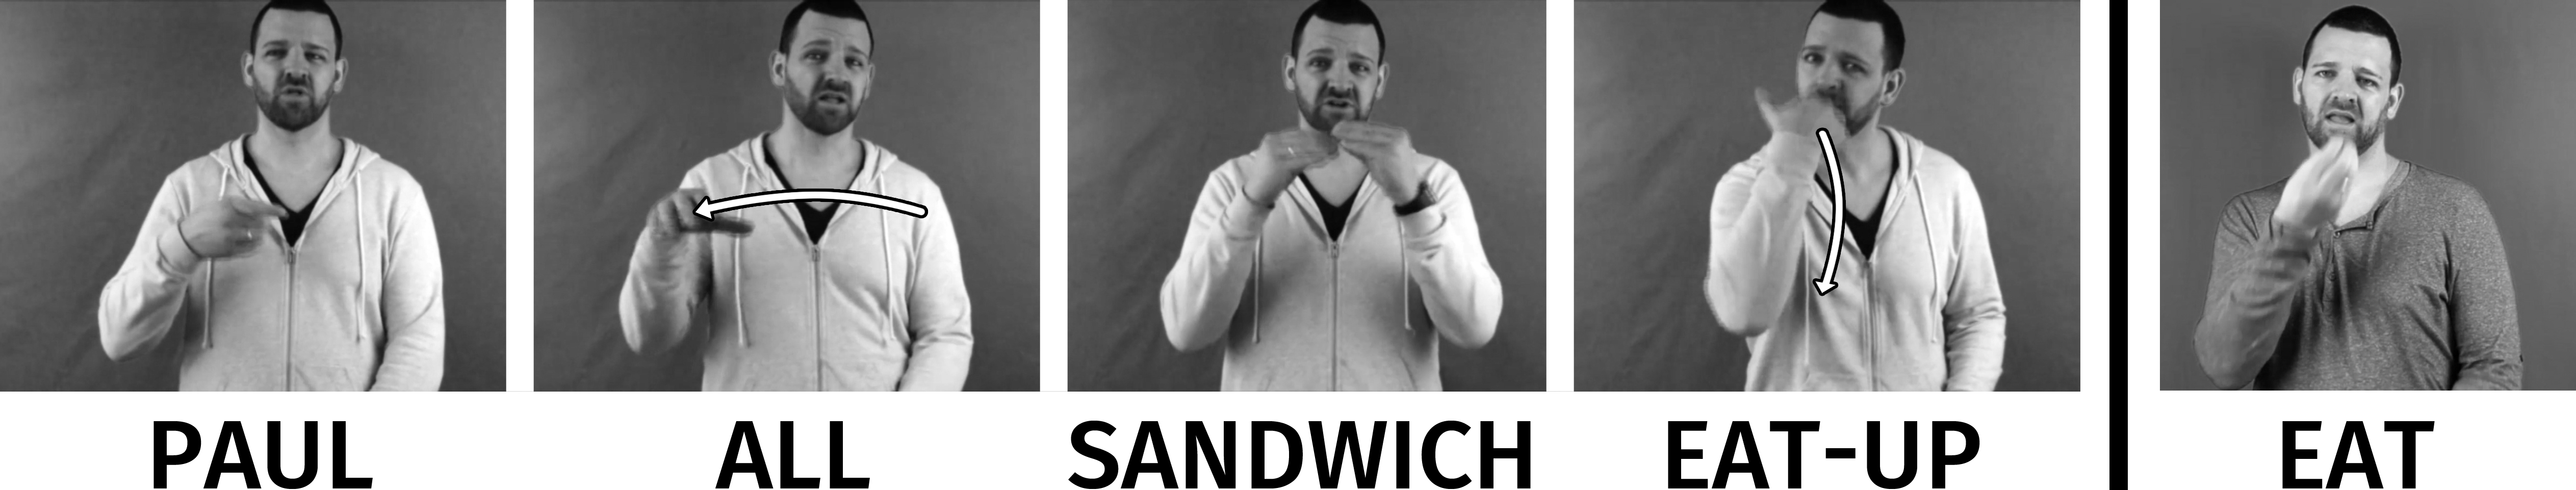
\includegraphics[width=\textwidth]{aufessensw.jpg}
	\caption{With completive II we find incorporation into the verb sign. In this case, the handshape of the sign \textsc{eat} is manipulated. The unmarked version of this sign is depicted on the right (separated by a thick black line). See also the distributive reading of \textsc{eat} in Figure \ref{fig:completiveonedgs} on page \pageref{fig:completiveonedgs}.}
	\label{labelfigure}
\end{figure}

\noindent Additionally, celerative I and celerative II can be combined in one clause -- another indication that we are dealing with two meanings.

\is{celerative aspect II|(}

\largerpage[-2]
\section{Completive aspect II (\textit{completely})}\label{completivetwo}\is{completive aspect|(}
\subsection{General overview}
As discussed in Section \ref{completiveone} (see page \pageref{completiveone}), Cinque distinguishes between two or three completive aspects. However, it is not entirely clear which is which. I assume the lower completive II to be an instance of the completion of a process that leads to reaching a natural endpoint. This contrasts with the examples in Section \ref{completiveone}, which do not have a natural endpoint.


\begin{figure}[bt]
\centering
	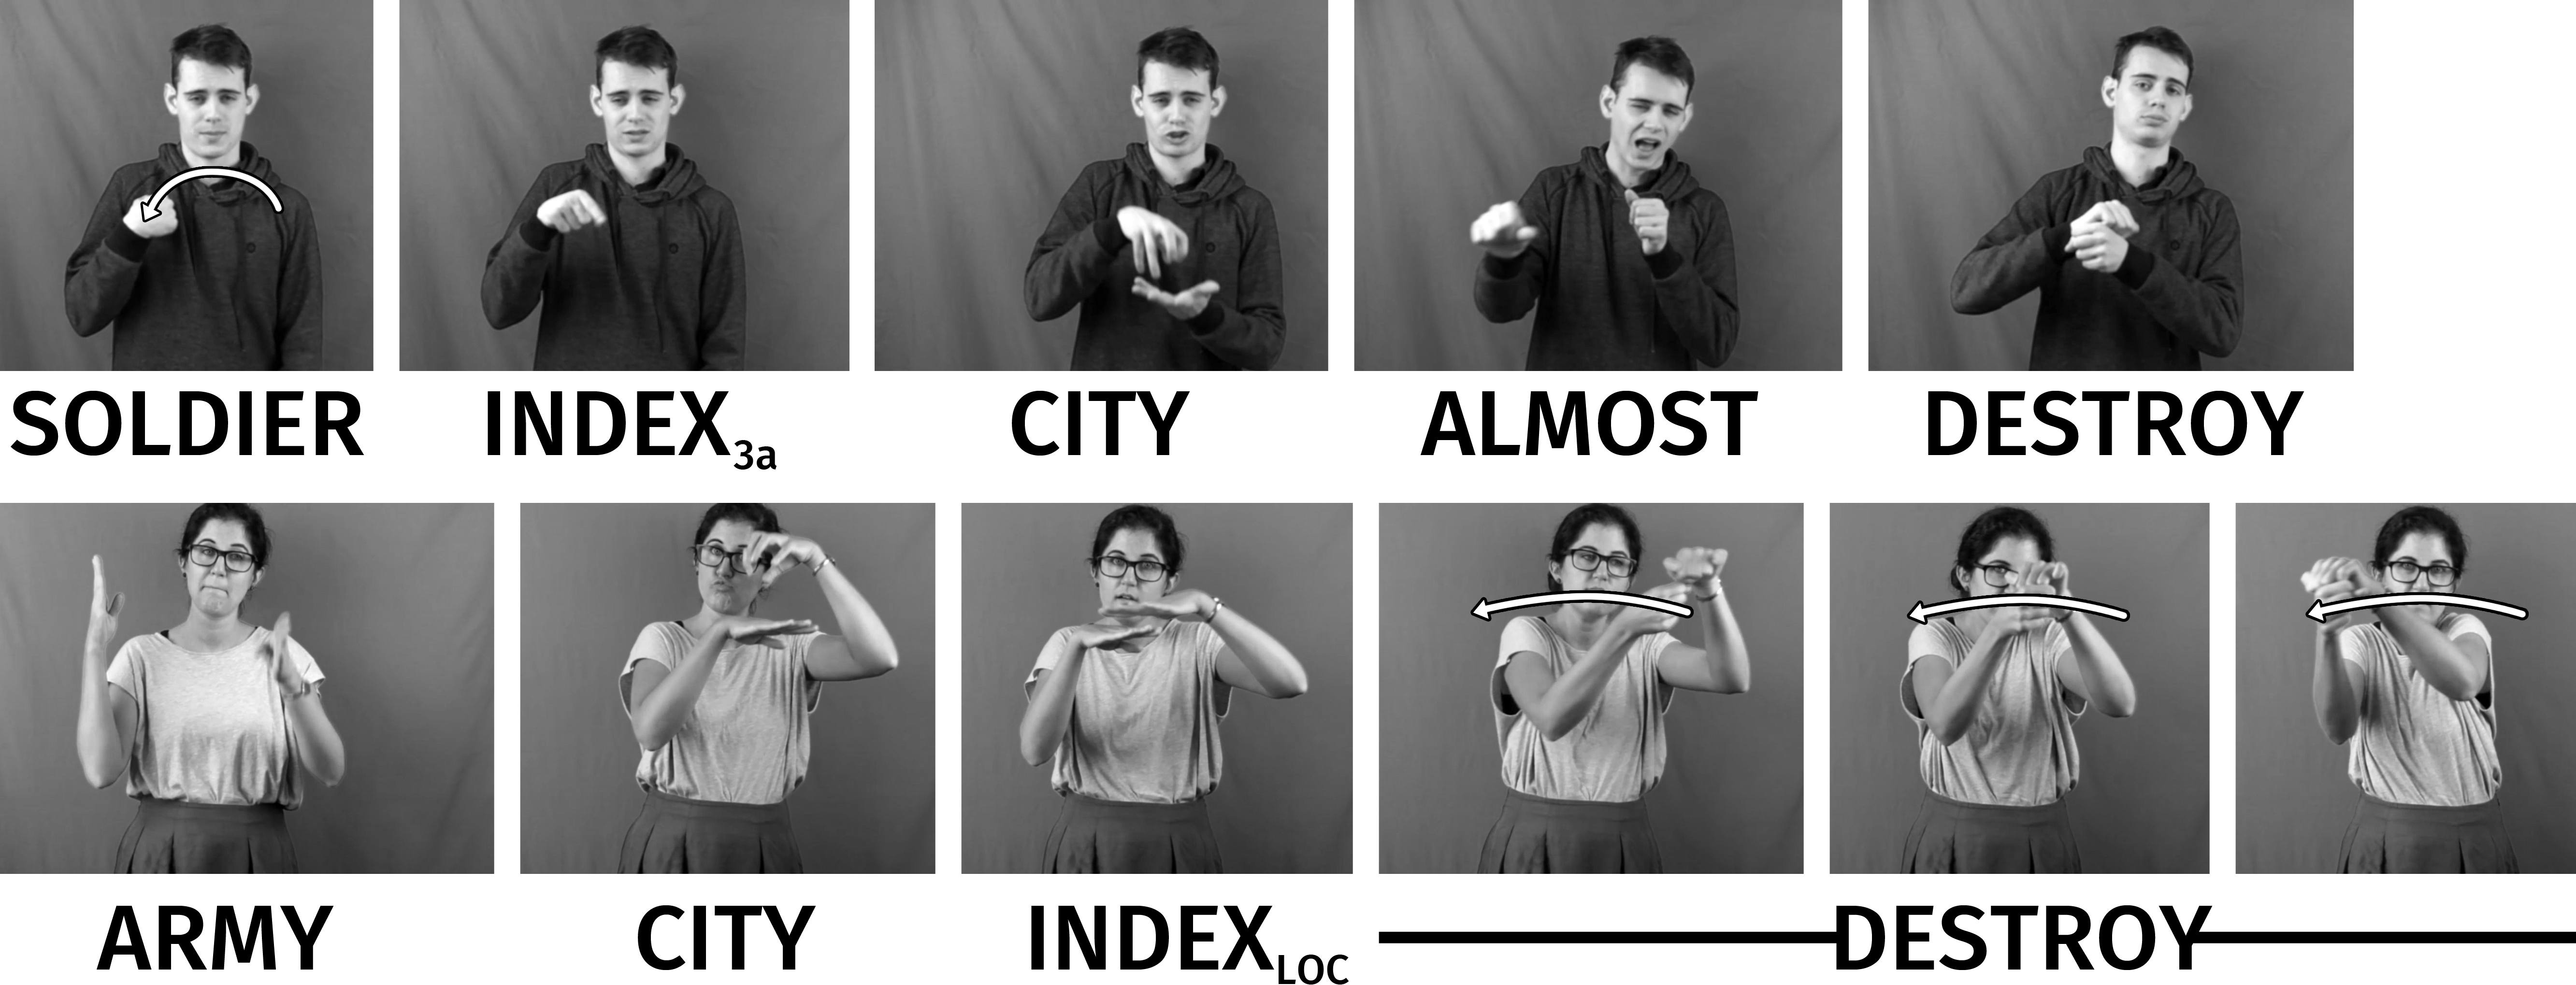
\includegraphics[width=1.0\textwidth]{completivetwosw.jpg}
	\caption{The two examples translate to \textit{The soldiers almost destroyed the city} (top) and \textit{The army completely destroyed the city} (bottom).}
	\label{fig:completivetwodgsexampletwo}
\end{figure}


\subsection{The situation in DGS}
As predicted, completive II is realized by modification of the verb. I will give two illustrative examples. The first example refers to a process in which all the sandwiches in the context are affected completely in that they are all eaten up. This is depicted in Figure \ref{labelfigure}. In this case, the hand shape and the way of execution of the verb sign \textit{eat} is altered in that the hand is open and the movement of the verb does not stop at the mouth, but proceeds to the chest (the left part of the image shows the actual example, the sign on the right is the normal sign \textsc{eat} not marked for aspect).

The second example refers to the destruction of a city and is depicted in Figure \ref{fig:completivetwodgsexampletwo}. The figure illustrates that the verbal sign \textsc{destroy} when not inflected for aspect refers to a point, as shown by the top example (`The soldiers almost destroyed the city'). When the object of the destruction, however, is completely affected, then this information is incorporated into the verbal sign. In this case (`The army completely destroyed the city', the second example in the figure), the verb is signed in the part of the signing space in which the city had been located previously by an locational index. It is not clear yet how completive II is realized with body-anchored verbs. I will leave this question open for future studies.
\newpage



\begin{digression}{{A note on \textsc{finish}, \textsc{through} and perfective aspect}}{}
\noindent \label{exkursfertigdurch}A very similar, though distinct, meaning can be achieved by the perfective marker \textsc{finish} that marks a proposition as being without interior composition, as shown in (\ref{dgsfinish}). In this example, the reading of the book is also understood as being completed. It seems, however, that \textsc{finish} rather marks perfective aspect than completive aspect similar to what has been described for \is{American Sign Language}American Sign Language (e.g., \citealt{aarons1992clausal}) or \is{Italian Sign Language}Italian Sign Language (e.g., \citealt{zucchi2003}). However, it seems that the use of \textsc{finish} also seems to have a meaning of completive aspect in some sign languages (e.g., \citealt{meir1999aperfect} on \is{Israeli Sign Language}Israeli Sign Language). A similar meaning as the one contributed by the sign \textsc{finish} in DGS can be achieved by another clause-final element, that I glossed \textsc{through} in (\ref{dgsthrough}).


\begin{exe}
\ex\label{ex:perfectivea}\begin{xlist}
\ex{\textsc{paul book read finish}}
\glt `Paul read the book.' \label{dgsfinish}
\ex{\textsc{paul book read through}}
\glt `Paul read through the book.' \label{dgsthrough}
\end{xlist}
\end{exe}

\noindent The sign \textsc{through} is also described in \citet[259]{rathmann2005event}, however as a continuative marker. It is still unclear if the sign described by Rathmann and the sign discussed here are the same as Rathmann has no picture of it and does not describe how it is performed. It could, however, be that we are dealing with two different signs, as \textsc{through} in the example in (\ref{dgsthrough}) seems to have a different meaning than the one described by Rathmann. Thus more research is needed. Both signs, \textsc{finish} and \textsc{through}, are depicted in the following figure: \\

\begin{center}
	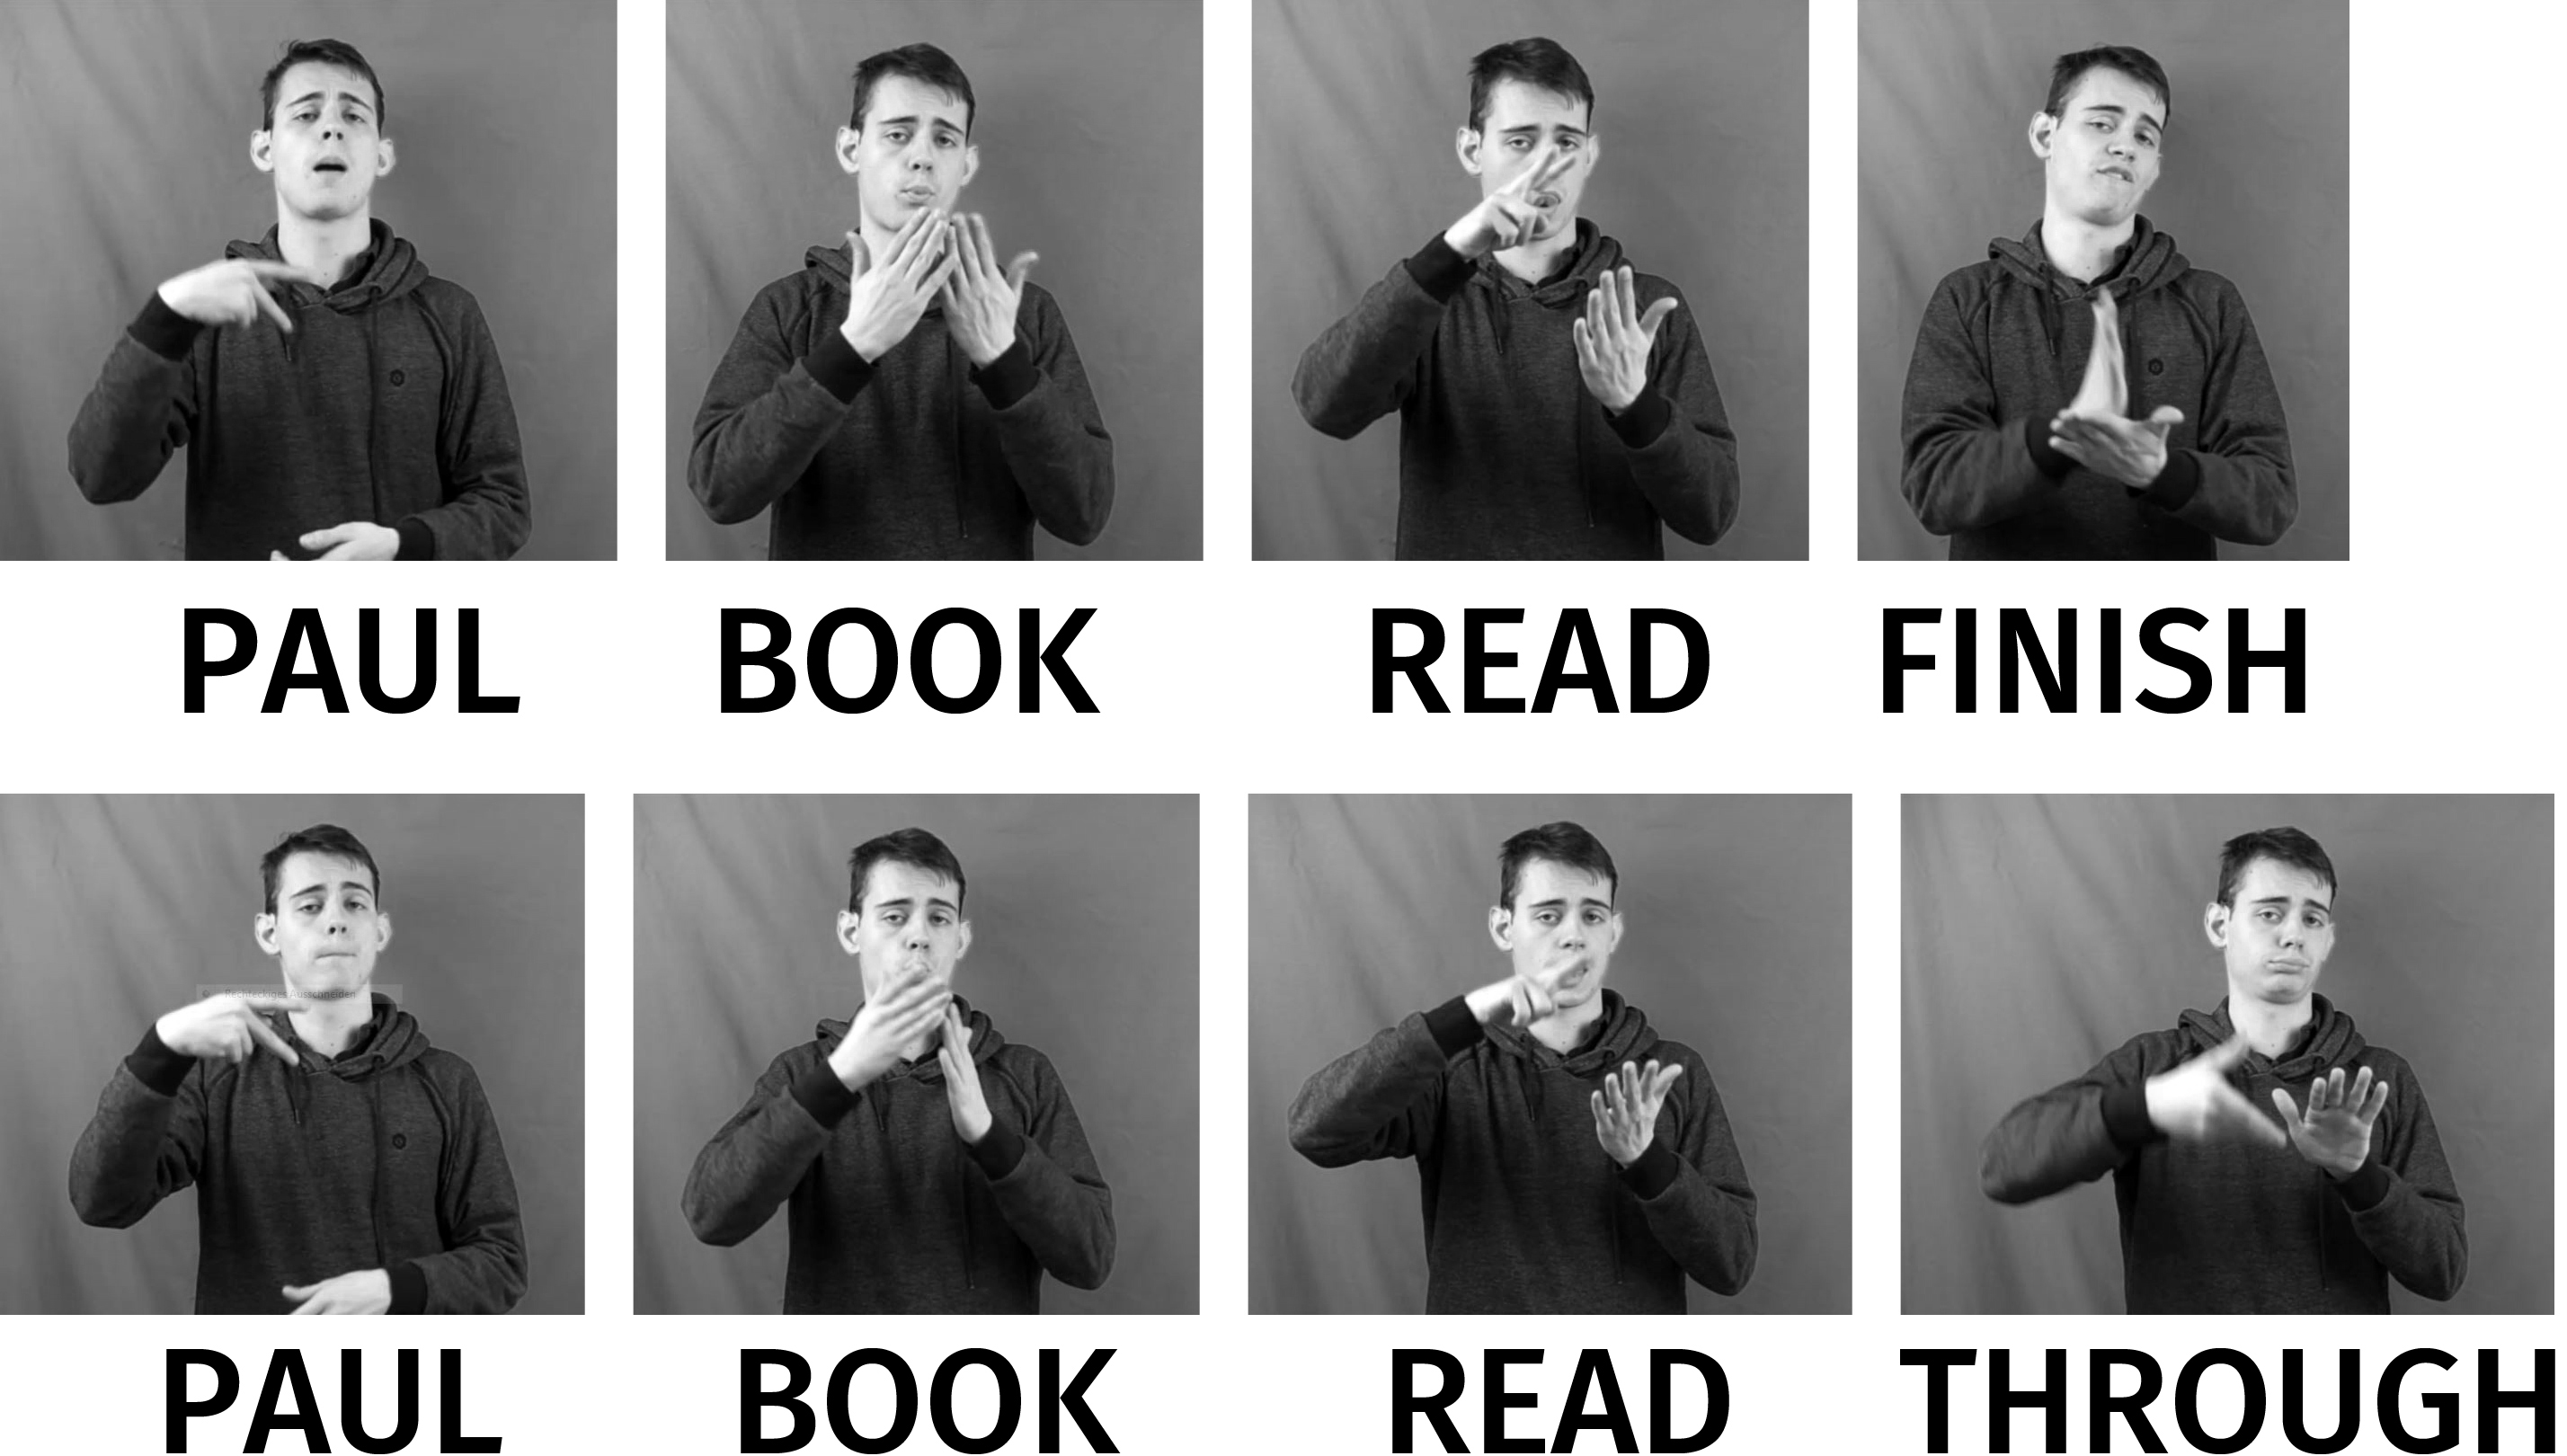
\includegraphics[width=0.5\textwidth]{fertigunddurchsw.jpg}
	\end{center}
	%\caption{Testcaption}
	%\label{fig:throughfinish}
\newpage

\noindent Note that the perfective marker \textsc{finish} is usually described to be restricted to occurring in a clause-final position in the literature (e.g., \citealt[3]{pfau2004grammaticalization}; \citealt[261--262]{rathmann2005event}). However, I often found \textsc{finish} in a pre-verbal position. It is yet unclear if this leads to differences in meanings as has been described for \is{American Sign Language}American Sign Language (see \citealt{rathmann2005event}). It is also unclear how to model this syntactically. It may also turn out that \textsc{finish} is located in a small clause\is{small clause}.
% \vspace*{-1cm}
%\end{theo}
\end{digression}




\section{Repetitive aspect II (\textit{again})}\label{repetitivetwo}\is{repetitive aspect II|(}
\subsection{General overview}
\is{completive aspect|(}
While repetitive aspect I refers to the iteration of an event on a single occasion (see Section \ref{repetitiveonesection} on page \pageref{repetitiveonesection}), repetitive II refers to the iteration of a process. In contrast to frequentative aspect which refers to several repetition (\textit{often}), repetitive aspect is about a single iteration (\textit{again}, \textit{once more}).

\subsection{The situation in DGS}
It would be easy to imagine that repetitive aspect II finds its expression in repeating the verb sign: a plausible scenario would involve first signing the verb, making a short pause, and signing it again to indicate that the process repeated (the two processes would  then refer to one single event). However, this is not what we find. It is either manually indicated how often the process was repeated (e.g., twice) or the verb is repeated two times, but the manual adverb \textsc{again} is sandwiched in between the two verbs, as shown in (\ref{ggsrepetitivetwo}).


\begin{exe}
\ex {\textsc{paul door knock, again knock}}
\glt `Paul knocks on the door again.' \label{ggsrepetitivetwo}
\end{exe}

\noindent As the example shows, there is a pause after the first instance of \textsc{knock} that leads to the impression that we are not dealing with some kind of grammaticalized sandwich structure, but rather with two clauses (\textit{Paul knocked at the door and then knocked again}). Therefore, I conclude, that repetitive aspect II is not grammaticalized in DGS.
\is{repetitive aspect II|(}




\section{Frequentative aspect II (\textit{often})}\label{frequentatitivetwo}\is{frequentative aspect II|(}
\subsection{General overview}
As was noted in Section \ref{frequentative}, frequentative aspect I is expressed by using the (left-to-right concatenated) manual sign \textsc{often}. Examples for frequentative I are, for convenience, given in (\ref{ex:freqaspIa}) and (\ref{ex:freqaspIb}) again. In this case, the event of insulting occurs frequently, for example, every day. This means that the event occurs frequently on different occassions.

\begin{exe}
\ex\begin{xlist}
\ex[]{\textsc{paul pam maria often insult}
\glt `Paul insults Maria often.' \label{ex:freqaspIa}}
\ex[*]{\textsc{paul pam maria insult often}
\glt `Paul insults Maria often.' \label{ex:freqaspIb}}
\end{xlist}
\end{exe}

\noindent With frequentative II, the event also occurs frequently, but on one occasion. \citet[92]{cinque1999adverbs} illustrates this difference with Italian adverb \textit{spesso} that can occur in two different positions, as shown in (\ref{ex:cinquefreqa}) and (\ref{ex:cinquefreqb}). The two different positions can be easily identified by its relative position to \textit{già} `already' in the examples.

\begin{exe}
\ex Italian \citep[92]{cinque1999adverbs}\begin{xlist}
\ex {(Quando troviamo qualcosa) questa è \textit{spesso già} stata scoperta da qualcuno.} \\
`(When we find something) that has often already been discovered by someone.' \label{ex:cinquefreqa}
\ex {Questa proprietà è \textit{già} stata scoperta \textit{spesso}, negli ultimi cinquant'anni.} \\
`This property has already been discovered often, in the last fifty years.' \label{ex:cinquefreqb}
\end{xlist}
\end{exe}


\noindent As the examples show, \textit{spesso} in its higher position, in (\ref{ex:cinquefreqa}), refers to different events that are viewed as completed. The lower one, in contrast, refers to a frequency in one time interval as in (\ref{ex:cinquefreqb}). Cinque assumes that there are not two different \textit{spesso}, but that they occupy two different (scope) positions in the clause. Note that both positions can be filled in one clause, as exemplified in (\ref{ex:cinquefreqc}), taken from \citet[92]{cinque1999adverbs}.

\begin{exe}

\ex Italian \citep[92]{cinque1999adverbs} \\ {Gianni saggiamente, \textit{spesso} esce con la stessa persona \textit{spesso}.}
\glt `Gianni, wisely, often dates the same person often.' \label{ex:cinquefreqc}

\end{exe}


\subsection{The situation in DGS}
\noindent In DGS, \textsc{often} cannot be used for expressing frequentative II. Instead, we find a \is{reduplication}reduplication of the verbal sign, as illustrated in (\ref{ex:freqaspIIa}). With this, DGS behaves similar to \is{American Sign Language}American Sign Language as described by \citet{klima1979signs,rathmann2005event}; see also \citet{pfausteinbwol2012tense} where this category has also been labeled `iterative aspect'.\is{iterative aspect}

Note that the reduplication in (\ref{ex:freqaspIIa}) does not consist of a single repetition of the sign, but of several repetitions, sometimes with short pauses between the repetitions \citep[163]{papaspyrou2008grammatik}. Additionally, \textsc{often} and the reduplication of the verb sign can easily combine into one sentence, as shown in (\ref{ex:freqaspIIb}).


\begin{exe}
\ex\label{frequecsaca}\begin{xlist}
\ex {\textsc{paul pam maria insult+++}}
\glt `Paul insults Maria often ($=$ many times on a single occasion).' \label{ex:freqaspIIa}
\ex {\textsc{paul pam maria often insult+++}}
\glt `Paul often insults Maria often.' \label{ex:freqaspIIb}
\end{xlist}
\end{exe}

\noindent Similar observations, namely that frequentative II involves the fast \is{reduplication}reduplication of the verb root, have been made for many sign languages (e.g., \citealt{bergmandahl1994, sutton1999linguistics, meir2007language} and seems to be a cross-linguistically stable pattern \citep[227]{signgram2017}.\footnote{ It could turn out in the end that at least some instances of what is often labeled `habitual aspect' in the literature and frequentative II are one and the same category. }

\is{frequentative aspect II|)}

\largerpage
\section{Summary and conclusion}
The discussion in this chapter has shown that the inner aspects taking scope below VoiceP indeed find their expression by manipulating the movement path of the verb sign. Additionally, I have argued that what is usually labeled habitual aspect in the sign language literature, a category expressed by \is{lower layering}lower layering, also belongs to the inner aspects. Evidence for this claim came from the fact that it is not possible to use this habitual aspect II with scope above modal verbs. A similar claim was made for the so called `durative'.

It is still unclear if these observations map one-to-one to other sign languages. However, similar patterns are attested even in spoken languages. In German, for example, frequentative I and frequentative II is expressed by the adverb \textit{oft} `often'. It is, however, also possible to add a bound morpheme to the verb to express frequentative II. The verb \textit{tropfen} `to drip', for example, can be transformed into \textit{tröpfeln} which expresses the existence of many drips at a single event time (therefore it is not possible to say *\textit{Der Wasserhahn wird ein mal tröpfeln} `The tap will drip one time.').\footnote{ Note that the suffix -\textit{eln} not only leads to an iterative, but also to a diminutive reading. Additionally, other meanings like `low intensity' can be contributed by the suffix (cf. \citealt{weidhaasschmid2015diminutiv}). The iterative meaning is, however, clearly added if the suffix is attached to an already existing verb. In other cases, when the suffix is used to derive a verb from an adjective, for example, sometimes only diminutive readings survive, as in \textit{krank} `sick' $\rightarrow$ \textit{kränk-eln}.} While using the adverb \textit{oft} can be equated with using a manual sign, the use of the bound morpheme can be equated with \is{lower layering}lower layering.

\begin{figure}[bt]
\centering
	\includegraphics[width=1.00\textwidth]{lowerlayeringsw.jpg}
	\caption{A comparison of outer and inner aspects. The comparison of continuative aspect I\is{continuative aspect I} (A) and continuative aspect II\is{continuative aspect II} (B), celerative aspect I\is{celerative aspect I} (C) and celerative aspect II\is{celerative aspect II} (D), completive aspect I\is{completive aspect I} (E) and completive aspect II\is{completive aspect II} (F), and frequentative aspect I\is{frequentative aspect I} (G) and frequentative aspect II\is{frequentative aspect II} (H) reveals that the inner aspects are formed by manipulating the movement path of the verb sign.}
	\label{fig:lowerlayering}
\end{figure}


Figure \ref{fig:lowerlayering} summarizes the findings by comparing the expression of the outer aspects (labeled with the number I by Cinque) and the inner aspects (labeled with the number II by Cinque). The figure shows examples of continuative aspect I\is{continuative aspect I} and II (A and B), \is{celerative aspect I}celerative aspect I and II (C and D), \is{completive aspect I}\is{completive aspect II}completive aspect I and II (E and F), as well as \is{frequentative aspect I}frequentative aspect I and II (G and H). Comparing the expressions of the IP-internal outer aspects with the VoiceP-internal inner aspects shows that each outer aspect is expressed by one separate sign (with the exception of completive I), while the inner aspects are formed as predicted by the VoiceP-internal modulation hypothesis, namely by manipulating the movement path of the verb sign.



%Regarding the inner aspects I have argued that they find their expression via lower layering, i.e., by manipulating the movement path of the verb sign. The two probably most controversial claims in this area were that what is usually called `habitual aspect' in the sign language literature is actually an instantiation of a lower VoiceP-internal category and that what is usually labeled \index{durative aspect}`durative aspect' is actually an instance of celerative II\index{celerative aspect II}. For the other inner aspects discussed by Cinque (1999, 2006) I have shown that they either find their expression by lower layering (continuative II\index{continuative aspect II}, celerative II\index{celerative aspect II}, completive II\index{completive aspect II}, frequentative\index{frequentative aspect II} II) or have no grammaticalized expression in DGS at all (inceptive \index{inceptive aspect II}II, repetitive\index{repetitive aspect II} II).


%It is still unclear if these observations map one-to-one to other sign languages. However, similar patterns are attested even in spoken languages. In German, for example, frequentative I and frequentative II is expressed by the adverb \textit{oft} `often'. It is, however, also possible to add a bound morpheme to the verb to express frequentative II. The verb \textit{tropfen} `to drip', for example, can be transformed into \textit{tr\"opfeln} which expresses the existence of many drips at a single event time. While using the adverb \textit{oft} can be equated with using a manual sign, the use of the bound morpheme can be equated with \is{lower layering}lower layering.

%With this, I end the discussion of the Cinquean categories. I will now discuss the behavior of the direct object in DGS and thus descend the tree even further, namely to the position in the tree in which the syntactic object is base-generated. In the following sections I will discuss object shift and differential object marking in DGS.

